% Created 2019-09-05 jue 19:02
\documentclass[presentation,aspectratio=169]{beamer}
\usepackage[utf8]{inputenc}
\usepackage[T1]{fontenc}
\usepackage{fixltx2e}
\usepackage{graphicx}
\usepackage{longtable}
\usepackage{float}
\usepackage{wrapfig}
\usepackage{rotating}
\usepackage[normalem]{ulem}
\usepackage{amsmath}
\usepackage{textcomp}
\usepackage{marvosym}
\usepackage{wasysym}
\usepackage{amssymb}
\usepackage{hyperref}
\tolerance=1000
\usepackage{khpreamble}
\usepackage{amssymb}
\DeclareMathOperator{\shift}{q}
\DeclareMathOperator{\diff}{p}
\usetheme{default}
\author{Kjartan Halvorsen}
\date{2019-09-05}
\title{Computerized Control - analysis of discrete-time systems}
\hypersetup{
  pdfkeywords={},
  pdfsubject={},
  pdfcreator={Emacs 25.3.50.2 (Org mode 8.2.10)}}
\begin{document}

\maketitle


\section{Intro}
\label{sec-1}
\begin{frame}[label=sec-1-1]{Result from quizz}
\begin{itemize}
\item Very good results!
\item Nyquist plot + criterion
\item Robustness
\end{itemize}
\end{frame}
\section{Pole placement}
\label{sec-2}
\begin{frame}[label=sec-2-1]{Pole-placement and time-response}
Pair the pole-placement with the correct time-response (from HW1)
\begin{columns}
\begin{column}{0.4\textwidth}
\begin{center}
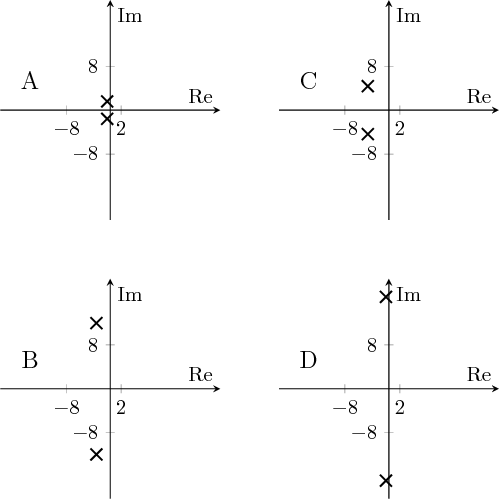
\includegraphics[width=\linewidth]{../../figures/pzmap-apollo}
\end{center}
\end{column}
\begin{column}{0.6\textwidth}
\begin{center}
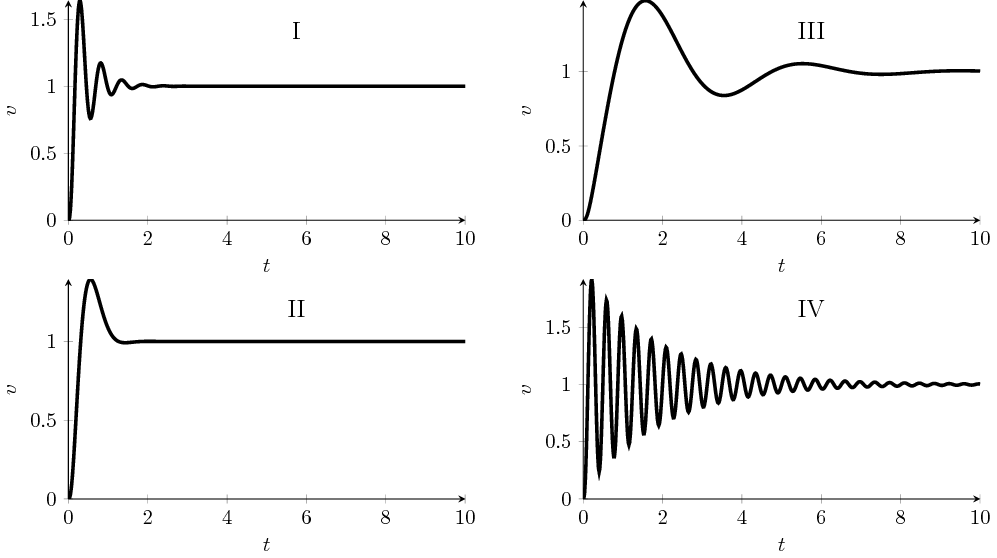
\includegraphics[width=\linewidth]{../../figures/step-response-apollo}
\end{center}
\end{column}
\end{columns}
\end{frame}

\begin{frame}[label=sec-2-2]{Mapping of poles from continuous time to discrete time}
\begin{center}
\begin{tabular}{ll}
Continuous time & Discrete time\\
\hline
\(Y(s) \triangleq \laplace{y(t)}\) & \(Y(z) \triangleq \ztrf{y(kh)}\)\\
\( Y(s) = G(s)U(s) = \frac{b}{s+a}U(s)\) & \(Y(z) = H(z)U(z) = \frac{\beta}{z+\alpha}U(z)\)\\
Pole of the system: \(s+a=0 \; \Rightarrow \; s = -a\) & Pole of the system: \( z+\alpha = 0 \; \Rightarrow \; z = -\alpha \)\\
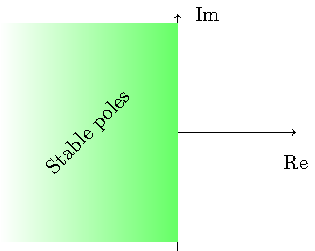
\includegraphics[width=0.22\linewidth]{../../figures/cont-stable} & 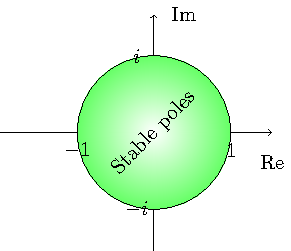
\includegraphics[width=0.22\linewidth]{../../figures/discrete-stable}\\
\hline
\end{tabular}
\end{center}

The \alert{s-domain} of continuous-time systems is related to the \alert{z-domain} of discrete-time systems as  \[z = \mathrm{e}^{sh}\]
\end{frame}

\begin{frame}[label=sec-2-3]{Mapping of poles from continuous time to discrete time}
Do excercise on paper!
\end{frame}

\section{Root locus}
\label{sec-3}


\begin{frame}[label=sec-3-1]{Root locus: A brief review}
\begin{center}
  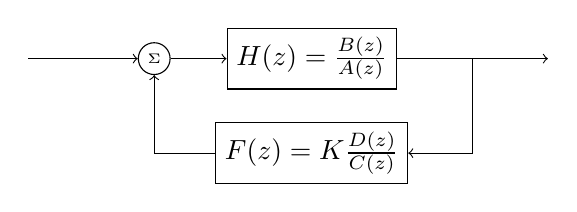
\begin{tikzpicture}[node distance=22mm, block/.style={rectangle, draw, minimum width=15mm}, sumnode/.style={circle, draw, inner sep=2pt}]
    
    \node[coordinate] (input) {};
    \node[sumnode, right of=input, node distance=16mm] (sum) {\tiny $\Sigma$};
    \node[block, right of=sum, node distance=20mm] (plant)  {$H(z)=\frac{B(z)}{A(z)}$};
    \node[block, below of=plant, node distance=12mm] (controller)  {$F(z)=K\frac{D(z)}{C(z)}$};
    \node[coordinate, right of=plant, node distance=30mm] (output) {};

    \draw[->] (input) -- node[above, pos=0.3] {} (sum);
    \draw[->] (sum) -- node[above] {} (plant);
    \draw[->] (plant) -- node[coordinate] (measure) {} node[above, near end] {} (output);
    \draw[->] (measure) |- (controller);
    \draw[->] (controller) -| (sum);
  \end{tikzpicture}
\end{center}

\begin{itemize}
\item The loop pulse-transfer function (loop gain) becomes \(L(z) = H(z)F(z) = K\frac{\overbrace{B(z)D(z)}^{Q(z)}}{\underbrace{A(z)C(z)}_{P(z)}} = K \frac{Q(z)}{P(z)}\).
\item The roots of \(Q(z)\) are called the \alert{open loop zeros}.
\item The roots of \(P(z)\) are called the \alert{open loop poles}.
\item The characteristic equation for the closed-loop system is \[ 1 + K\frac{Q(z)}{P(z)} = 0 \quad \Leftrightarrow \quad P(z) + KQ(z) = 0\]
\end{itemize}
\end{frame}


\begin{frame}[label=sec-3-2]{Root locus: Definition}
Let
\[\begin{cases} P(z)&=z^n+a_1z^{n-1}+\dots+a_n = (z-p_1)(z-p_2)\cdots(z-p_n)\\ 
Q(z)&=z^m+b_1 z^{m-1}+\dots+b_m=(s-q_1)(z-q_2)\cdots(z-q_m) \end{cases},\ \ \ n\ge m \]

The root locus shows how the \alert{solution} to the characteristic equation
\begin{equation}
\label{eq:P(z)+KQ(z)=0}
P(z)+K\cdot Q(z)=0,\ \ \ 0\le K<\infty
\end{equation}
depend on the parameter $K$. The root locus consists of the set of all points in the complex plane that are solutions to \eqref{eq:P(z)+KQ(z)=0} for some non-negative value of $K$.
\end{frame}

\begin{frame}[label=sec-3-3]{Root locus: Characteristics}
\begin{description}
\item[{Start points}] The \(n\) roots of \(P(z)\), marked by crosses
\item[{End points}] The \(m\) roots of \(Q(z)\), marked  by circles
\item[{Asymptotes}] Number equal to the \emph{pole excess} \(n-m\)
\item[{Real axis}] Some segments of the real axis belong to the root locus
\end{description}
\end{frame}

\begin{frame}[label=sec-3-4]{Root locus: Direction of the asymptotes}
The characteristic equation \(P(z)+K Q(z)=0\) can be written \(\frac{P(z)}{Q(z)} = -K\) and for large $z$ it can be approximated as 
\[ \frac{z^n}{z^m} = -K \quad \Leftrightarrow \quad z^{n-m} = -K.\]

Taking the argument of both sides of the equation gives 
\( (n-m)\arg z = \pi + k2\pi, \; k \in  \mathbb{Z} \)
So, the \alert{directions} of the asymptotes are given by the expression
\[ \theta_k = \arg z = \frac{(2k+1)\pi}{n-m}, \; k \in \mathbb{Z} \]
\end{frame}

\begin{frame}[label=sec-3-5]{Root locus: The asymptotes' intersection with the real axis}
\[ z_{ip} = \frac{ \sum_{i=0}^n p_i - \sum_{i=0}^m q_i}{n-m}, \]
where $\{p_i\}$ are the starting points (open-loop poles) and $\{q_i\}$ are the end points (open-loop zeros). 
\end{frame}

\begin{frame}[label=sec-3-6]{Root locus exerise: Pair the pulse-trf fcn and root locus}
\begin{columns}
\begin{column}{0.35\textwidth}

 \small
\begin{align*}
  G_1(z) &= K\frac{(z+2.9)(z+0.2)}{(z-1)^2(z-0.3)}\\[3mm]
  G_2(z) &= K\frac{(z-0.5)(z+0.4)}{(z-1)(z-0.3)(z-0.1)}\\[3mm]
  G_3(z) &= K\frac{(z-0.5)(z+0.8)}{(z-1)^2(z-0.3)}\\[3mm]
  G_4(z) &= K \frac{z-0.6}{(z-1)(z-0.3)}
\end{align*}
\end{column}

\begin{column}{0.65\textwidth}
\begin{center}
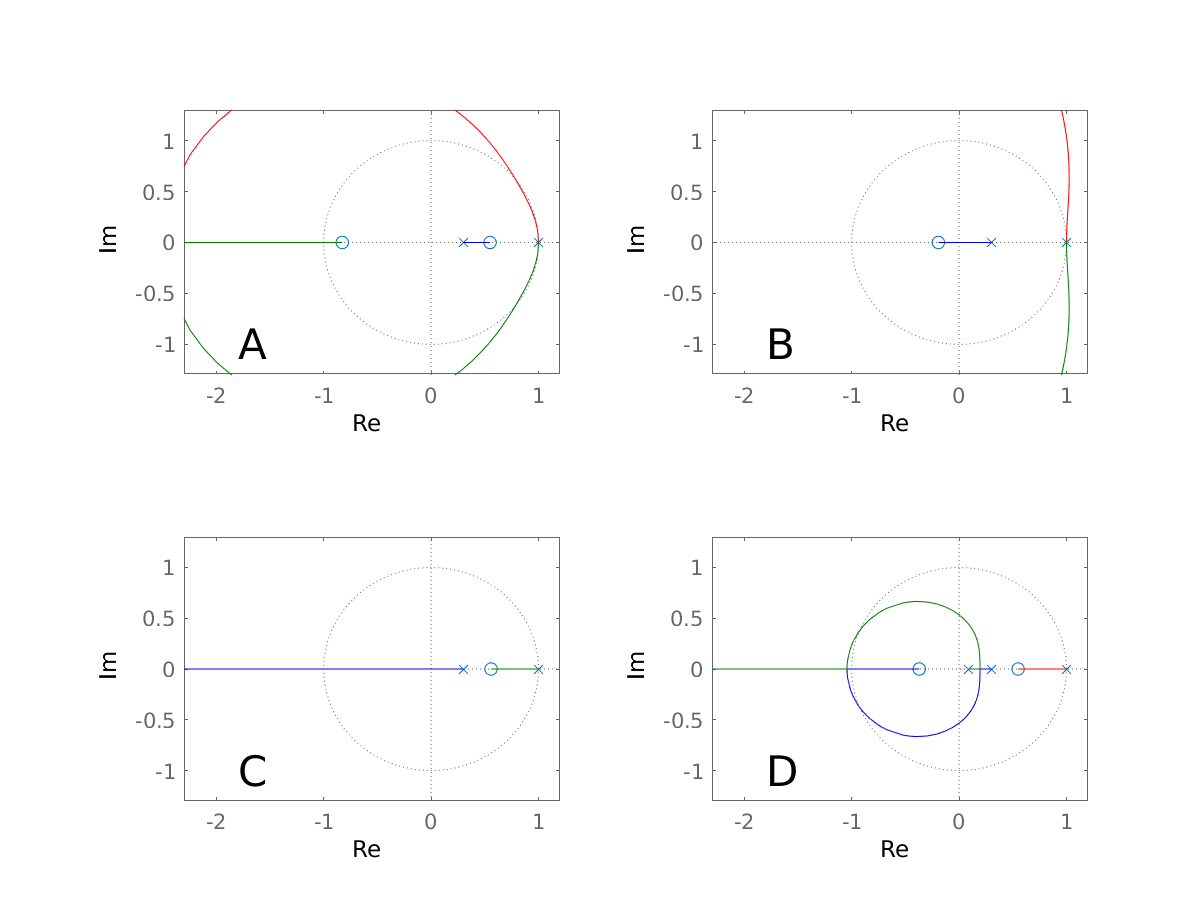
\includegraphics[width=1.04\linewidth]{../../matlab/rlocus_2x2-crop}
\end{center}
\end{column}
\end{columns}
\end{frame}


\begin{frame}[label=sec-3-7]{Draw a root locus}
Level control in a hydro power plant dam

\begin{center}
\small
\def\svgwidth{0.5\linewidth}
\input{hydroplant.pdf_tex}
\end{center}

Discrete-time model: \(y(k+1) - y(k) = \frac{h}{A} u(k) + \frac{h}{A}v(k)\), where \(y(k)\) is the deviation in water level from a standard level, \(u(k)\) is the (negative) deviation in flow through the dam ports and \(v(k)\) is a deviation in other flows (disturbance). 
\end{frame}

\begin{frame}[label=sec-3-8]{What happens if the poles are \alert{on the} unit circle?}
Say, in \(z = \mathrm{e}^{\pm i \omega_0}\)
\begin{center}
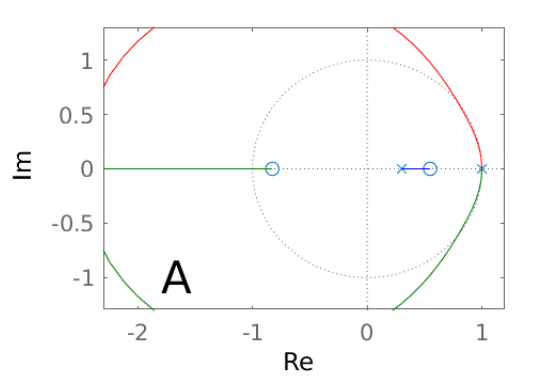
\includegraphics[width=0.3\linewidth]{../../figures/rlocusA.png}
\end{center}

\[H_c(z) = \frac{k z}{(z-\mathrm{e}^{i \omega_0})(z-\mathrm{e}^{-i \omega_0})} \overbrace{+ \cdots}^{\text{stable term}}\].
\end{frame}

\begin{frame}[label=sec-3-9]{What happens if the poles are \alert{on the} unit circle?}
Say, in \(z = \mathrm{e}^{\pm i \omega_0}\)
\begin{center}
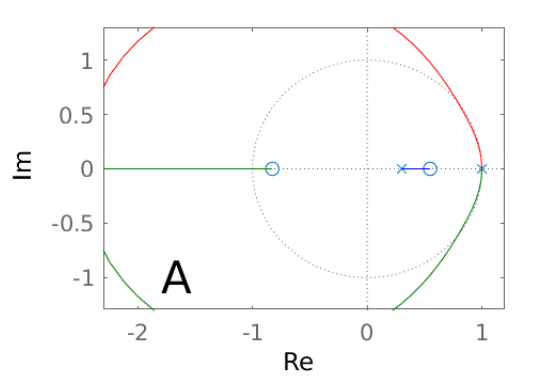
\includegraphics[width=0.3\linewidth]{../../figures/rlocusA.png}
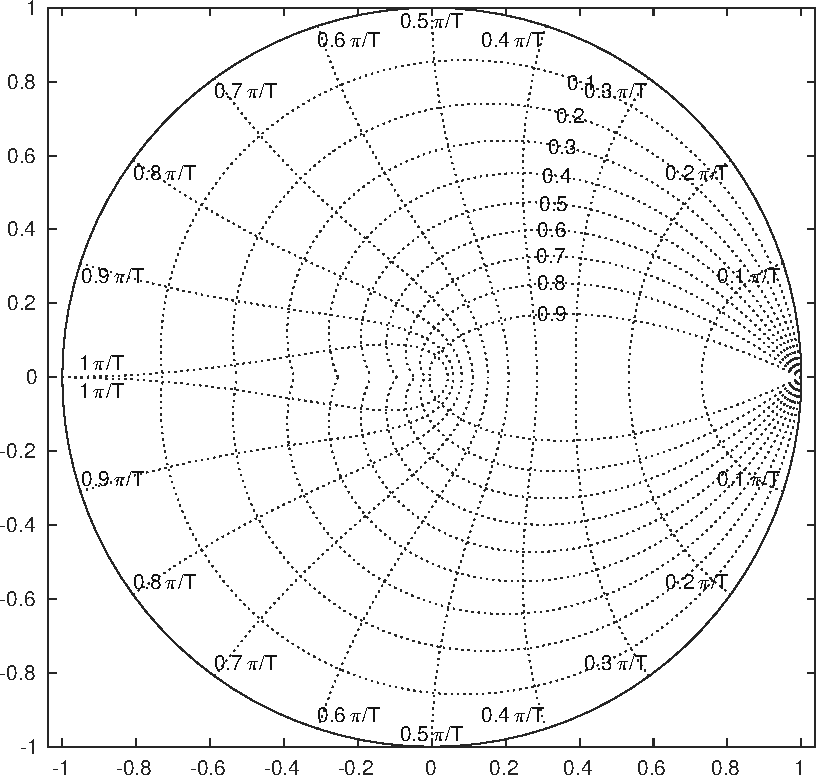
\includegraphics[height=0.34\textheight]{../../figures/zgrid-crop}\\
\end{center}

\begin{align*}
H_c(z) &= \frac{k z}{(z-\mathrm{e}^{i \omega_0})(z-\mathrm{e}^{-i \omega_0})} + \cdots\\
       &= \frac{k z}{z^2 -2\cos\omega_0 z + 1} + \cdots
\end{align*}

If \(\omega_0 = \frac{\pi}{6}\) and the sampling period is \unit{0.4}{\second}, what is the \alert{frequency} (in \unit{}{\radian\per\second} and in Hz) of the oscillations in the pulse response?
\end{frame}

\section{Bode diagrams and Nyquist plots}
\label{sec-4}
\begin{frame}[label=sec-4-1]{Bode diagram and Nyquist plots}
\end{frame}

\begin{frame}[label=sec-4-2]{Sine in --- sine out}
\begin{center}
  \begin{tikzpicture}[node distance=22mm, block/.style={rectangle, draw, minimum width=15mm}, sumnode/.style={circle, draw, inner sep=2pt}]
    
    \node[coordinate] (input) {};
    \node[block, right of=sum, node distance=25mm] (plant)  {$H(z)$};
    \node[coordinate, right of=plant, node distance=40mm] (output) {};
    
    \draw[->] (input) -- node[above, pos=0.3] {$u(kh) = \sin(\omega kh)$} (plant);
    \draw[->] (plant) -- node [above, pos=1.1] {$y(kh) = |H(\mathrm{e}^{i\omega h})|\sin(\omega kh + \arg H(\mathrm{e}^{i\omega h}))$} (output);
  \end{tikzpicture}
\end{center}
\end{frame}
\begin{frame}[label=sec-4-3]{Sine in --- sine out}
\begin{center}
  \begin{tikzpicture}[node distance=22mm, block/.style={rectangle, draw, minimum width=15mm}, sumnode/.style={circle, draw, inner sep=2pt}]
    
    \node[coordinate] (input) {};
    \node[block, right of=sum, node distance=25mm] (plant)  {$H(z)$};
    \node[coordinate, right of=plant, node distance=40mm] (output) {};
    
    \draw[->] (input) -- node[above, pos=0.3] {$u(kh) = \sin(\omega kh)$} (plant);
    \draw[->] (plant) -- node [above, pos=1.1] {$y(kh) = |H(\mathrm{e}^{i\omega h})|\sin(\omega kh + \arg H(\mathrm{e}^{i\omega h}))$} (output);
  \end{tikzpicture}
\end{center}
\alert{Prove it!} Some hints:
\begin{itemize}
\item Write \(\sin(\omega kh) = \mathrm{Im}\{\mathrm{e}^{i\omega kh}\}\).
\item Use \(H(z)U(z) \stackrel{\mathcal{Z}}{\leftrightarrow} h(k)\ast u(k)\), and write out the discrete-time convolution \(h \ast u = \sum_{n=-\infty}^\infty h(n)u(k-n) = \sum_{n=0}^\infty h(n)u(k-n) \)
\item Try to rewrite to obtain as a factor \(\sum_{n=0}^\infty h(n) \mathrm{e}^{-i\omega nh} = H(\mathrm{e}^{i\omega h})\).
\end{itemize}
\end{frame}


\section{Relative stability}
\label{sec-5}

\begin{frame}[label=sec-5-1]{The Nyquist plot}
Example of a \alert{Nyquist plot} or \alert{frequency curve}.
\begin{center}
  \begin{tikzpicture}
    \node at (0,0) {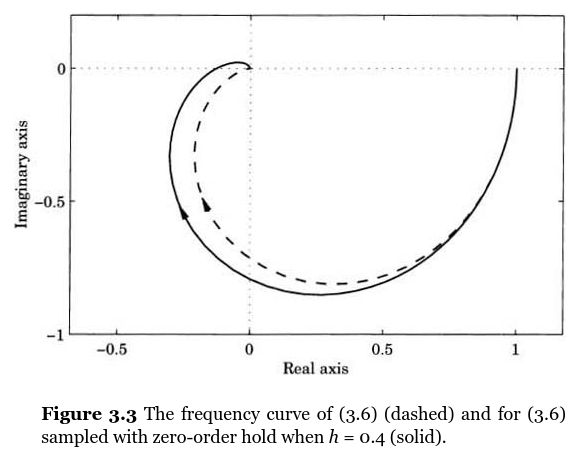
\includegraphics[width=0.4\linewidth]{../../figures/fig3-3.png}};
    \node[pin=120:{$H(z)$ evaluated at $z=\mathrm{e}^{i\omega h}$, $0<\omega<\frac{\pi}{h}$}] at (-1,1) {};
    \node[pin=40:{$G(s)$ evaluated at $s=i\omega$, $0<\omega<\infty$}] at (-0.98,0.4) {};
  \end{tikzpicture}
\end{center}



The system \(G(s) = \frac{1}{s^2 + 1.4s + 1}\) is sampled with ZOH-sampling (\(h=\unit{0.4}{\second}\)) to get \(H(z) = \frac{0.066z + 0.055}{z^2 - 1.45 z + 0.571}\)
\end{frame}

\begin{frame}[label=sec-5-2]{Simplified Nyquist criterion}
\begin{center}
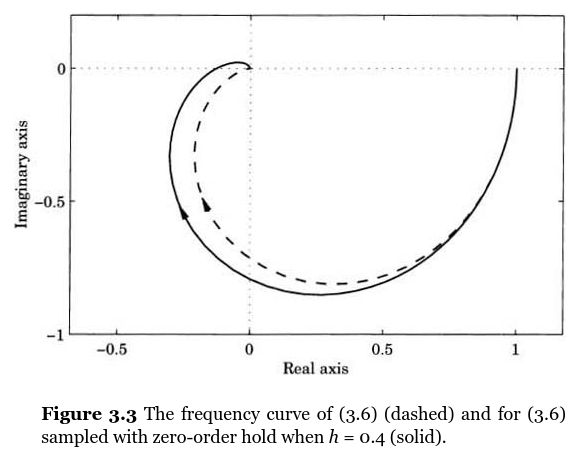
\includegraphics[width=0.4\linewidth]{../../figures/fig3-3.png}
\end{center}

Consider the loop pulse-transfer function $L(z)$ of a closed-loop system. If $L(z)$ is stable (no poles outside the unit circle), then the closed-loop system with characteristic equation $1 + L(z) = 0$ will be stable iff $L(z)$ evaluated on the unit circle (i.e, the Nyquist plot of $L$) has the point \alert{-1 to the left}.
\end{frame}

\begin{frame}[label=sec-5-3]{Stability margins - phase margin}
\begin{center}
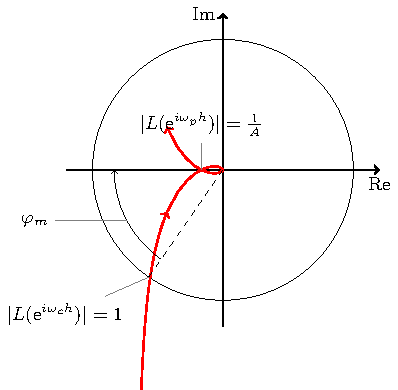
\includegraphics[width=0.38\linewidth]{../../figures/implane-nyquist-margins}
\end{center}
\begin{itemize}
\item Cross-over frequency: The frequency \(\omega_c\) for which \(|L(\mathrm{e}^{i\omega h})| = 1\).
\item Phase margin: The angle \(\varphi_m\) to the negative real axis for the point where the Nyquist curve intersects the unit circle. \[\varphi_m = \arg L(\mathrm{e}^{i\omega_c h}) - (-180\degree) = \arg L(\mathrm{e}^{i\omega_c h}) + 180\degree\]
\end{itemize}
\end{frame}

\begin{frame}[label=sec-5-4]{Stability margins - gain margin}
\begin{center}
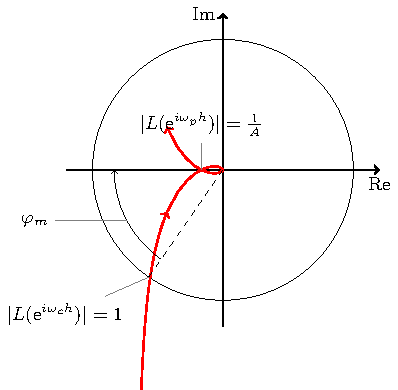
\includegraphics[width=0.34\linewidth]{../../figures/implane-nyquist-margins}
\end{center}
\begin{itemize}
\item phase-cross-over frequency: The frequency \(\omega_p\) for which \(\arg L(\mathrm{e}^{i\omega h}) = -180\degree\).
\item Gain margin: The gain $K=A$ that would make the Nyquist curve of \(K L(\mathrm{e}^{i\omega h})\) go through the point \(-1 + i0\). This means that \[ |L(\mathrm{e}^{i\omega_p h})| = \frac{1}{A}. \]
\end{itemize}
\end{frame}

\begin{frame}[label=sec-5-5]{The relationship between Bode diagrams and frequency curves (Nyquist plots)}
They are both showing the value of a pulse-transfer function $H(z)$ evaluated for $z = \mathrm{e}^{i\omega h}$, $0<\omega \le \frac{\pi}{h}$.

\begin{center}
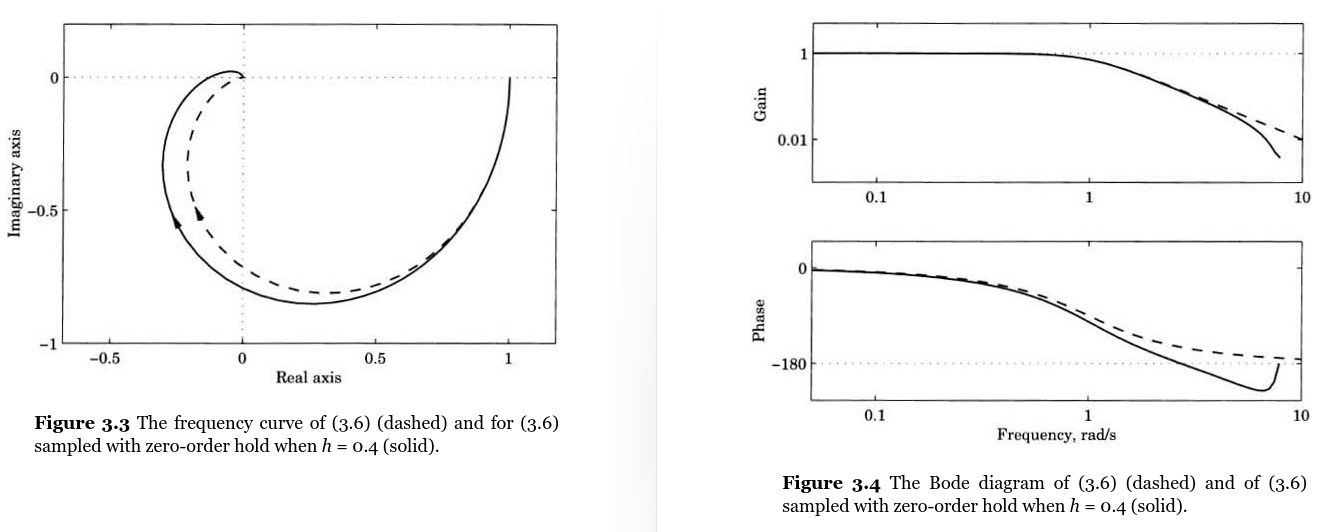
\includegraphics[width=\linewidth]{../../figures/fig3-3-4.png}
\end{center}
\end{frame}
% Emacs 25.3.50.2 (Org mode 8.2.10)
\end{document}